%% This is an example first chapter.  You should put chapter/appendix that you
%% write into a separate file, and add a line \include{yourfilename} to
%% main.tex, where `yourfilename.tex' is the name of the chapter/appendix file.
%% You can process specific files by typing their names in at the 
%% \files=
%% prompt when you run the file main.tex through LaTeX.
\chapter{Experiment}

\section{Setup}

All jobs were run using the spark interactive shell.
All jobs were run ten times, with the last five times being averaged.
All local jobs were run on a 2013 MacbookPro with 8GB of RAM 
All distributed jobs were run using the spark/ec2 launch scripts. They were run on 
four AWS m1.large machines in the us west zone. They were run ten times, with the last five times 
being average.

\section{Regular Shuffle}


\section{Broadcast and ShuffleJoinRDD}

For this test, we created a bigger RDD with key-value pairs of (x,2 * x) with x ranging from 1 to 100 milllion.
As seen in the Figure~\ref{fig:rddjoin}, we then then manipulated the number of key-value pairs of the smaller rdd, 
with each key value pairs being (x,x). We measured our the performance for the ShuffleJoinRDD and BroadcastJoinRDD. 
We ran this on AWS. As expected, initially the BroadcastJoinRDD performs better as it requires significantly network traffic.
However, it soon becomes slower then the ShuffleJoinRDD as it gets transmitted to every partition while in the ShuffleJoinRDD it
does not.

\begin{figure}[h]
\begin{center}
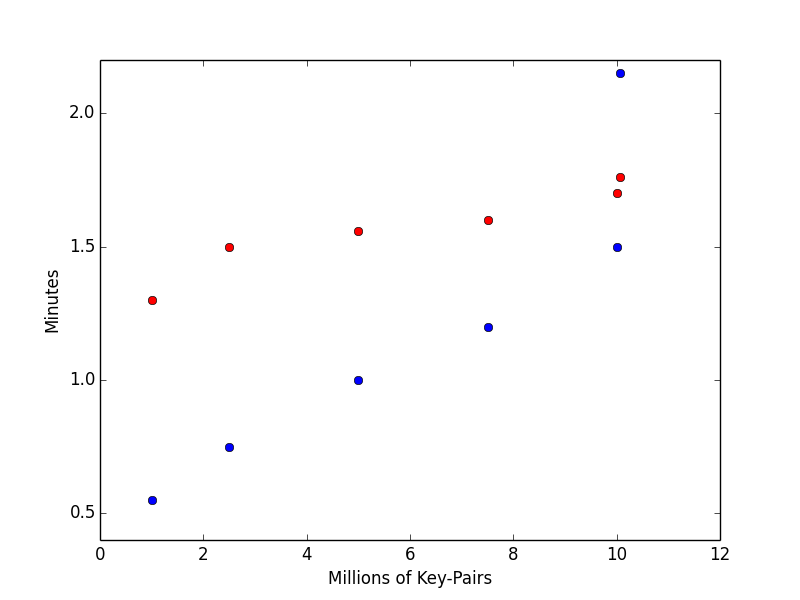
\includegraphics[scale=0.6]{./img/rddjoin.png}
\caption{BroadcastJoinRDD vs ShuffledJoinRDD}
\label{fig:rddjoin}
\end{center}
This figure measures the performance of joins complete using the BroadcastJoinRDD versus the ShuffleJoinRDD.
The BroadcastJoinRDD is in blue while the ShuffleJoinRDD is in red. The bigger rdd is fixed with 100 million key-value pairs,but the 
key-value pairs of the small RDD is manipulated along the x axis.
\end{figure}

\section{Spark SQL join}
